%%%%%%%%%%%%%%%%%%%%%%%%%%%%%%%%%%%%%%%%%%%%%%%%%%%%%%%%%%%%%%%%%%%%%%%%
%     LaTeX source code to approximate a NIST Technical report
%	  Instructions for authors: tinyurl.com/techpubsnist 
%	DOI watermark will be added on final PDF
% 	Developed by K. Miller, kmm5@nist.gov 
%	Last updated: 26-March-2019
%%%%%%%%%%%%%%%%%%%%%%%%%%%%%%%%%%%%%%%%%%%%%%%%%%%%%%%%%%%%%%%%%%%
\documentclass[12pt]{article}
\usepackage{adjustbox}
\usepackage{amsmath}
\usepackage{amsfonts}   % if you want the fonts
\usepackage{amssymb}    % if you want extra symbols
\usepackage{booktabs}
\usepackage{bm}
\usepackage{chemformula}
\usepackage{float}
%\usepackage{fourier}
\usepackage[hang,flushmargin,bottom]{footmisc} % footnote format
\usepackage{graphicx}   % need for figures
\usepackage{mathptmx}
\usepackage{multicol}
\usepackage{physics}
\usepackage{rotating}
\usepackage{secdot}
\usepackage{siunitx} % Formats the units and values
\usepackage{tabulary}
\usepackage{textgreek}
\usepackage{textcomp}
\usepackage{tikz}
\usepackage[newparttoc]{titlesec}
\usepackage[utf8]{inputenc}
\usepackage{xcolor}
\titleformat{\section}{\normalsize\bfseries}{\thesection.}{1em}{}	% required for heading numbering style
\titleformat*{\subsection}{\normalsize\bfseries}

\usepackage{tocloft}	% change typeset, titles, and format list of appendices/figures/tables
\renewcommand{\cftdot}{}	
\renewcommand{\contentsname}{Table of Contents}
\renewcommand{\cftpartleader}{\cftdotfill{\cftdotsep}} % for parts
\renewcommand{\cftsecleader}{\cftdotfill{\cftdotsep}}
\renewcommand\cftbeforesecskip{\setlength{4pt}{}}
\addtolength{\cftfignumwidth}{1em}
\renewcommand{\cftfigpresnum}{\figurename\ }
\addtolength{\cfttabnumwidth}{1em}
\renewcommand{\cfttabpresnum}{\tablename\ }
\setlength{\cfttabindent}{0in}    %% adjust as you like
\setlength{\cftfigindent}{0in} 

\usepackage{enumitem}         % to control spacing between bullets/numbered lists

\usepackage[numbers,sort&compress]{natbib} % format bibliography 
\renewcommand{\bibsection}{}
\setlength{\bibsep}{0.0pt}

\usepackage[hidelinks]{hyperref}
\hypersetup{
	colorlinks = true,
urlcolor ={blue},
citecolor = {.},
linkcolor = {.},
anchorcolor = {.},
filecolor = {.},
menucolor = {.},
runcolor = {.}
pdftitle={},%%put title here to auto-fill properties of the PDF
pdfsubject={},%%put abstract here
pdfauthor={}, %%put author list here
pdfkeywords={} %%put keywords here
}
\urlstyle{same}

\usepackage{epstopdf} % converting EPS figure files to PDF

\usepackage{fancyhdr, lastpage}	% formatting document, calculating number of pages, formatting headers
\setlength{\topmargin}{-0.5in}
\setlength{\headheight}{39pt}
\setlength{\oddsidemargin}{0.25in}
\setlength{\evensidemargin}{0.25in}
\setlength{\textwidth}{6.0in}
\setlength{\textheight}{8.5in}

\usepackage{caption} % required for Figure labels
\captionsetup{font=small,labelfont=bf,figurename=Fig.,labelsep=period,justification=raggedright} 

%%%%%%%%%%% !!!!!! REQUIRED - FILL OUT METADATA HERE !!!!!!!! %%%%%%%%%%%%%%
%  	Report Number - fill in Report Number sent to you (see info below)
%   DOI Statement - fill in DOI sent to you 
%   Month Year - fill in Month and Year of Publication
%%%%%%%%%%%%%%%%%%%%%%%%%%%%%%%%%%%%%%%%%%%%%%%%%%%%%%%%%%%%%%%%%%%%%%%%%%%%%%%%%%%%%%
\newcommand{\pubnumber}{XXXX}
\newcommand{\DOI}{https://doi.org/10.6028/NIST.TN.XXXX}
\newcommand{\monthyear}{August 2019}


\newcommand*\chem[1]{\ensuremath{\mathrm{#1}}}

\newcommand\numberthis{\addtocounter{equation}{1}\tag{\theequation}}

%%%%%%%%%%%%%%%%%%%%%%%%%%%%%%%%%%%%%%%%%%%%%%%%%%%%%%%%%%%%%%%%%%%%
%   	BEGIN DOCUMENT 
%%%%%%%%%%%%%%%%%%%%%%%%%%%%%%%%%%%%%%%%%%%%%%%%%%%%%%%%%%%%%%%%%%%%
\begin{document}
	\urlstyle{rm} % Format style of \url   
	
%%%%%%%%%%%%%%%%%%%%%%%%%%%%%%%%%%%%%%%%%%%%%%%%%%%%%%%%%%%%%%%%%%%%
%   Cover Page is REQUIRED and must contain the information 
%	displayed here, at a minimum. Additional artwork may be included 
%	(e.g., official project/conference logo, etc.).
%	Pub Number automated based on metadata
%%%%%%%%%%%%%%%%%%%%%%%%%%%%%%%%%%%%%%%%%%%%%%%%%%%%%%%%%%%%%%%%%%%%
	\begin{titlepage}
		\begin{flushright}
%%%%%%%%%%%%%%%%%%%%%%%%%%%%%%%%%%%%%%%%%%%%%%%%%%%%%%%%%%%%%%%%%%%%
% 	Automated based on metadata - delete if not applicable
%%%%%%%%%%%%%%%%%%%%%%%%%%%%%%%%%%%%%%%%%%%%%%%%%%%%%%%%%%%%%%%%%%%%
\LARGE{\textbf{NIST Technical Note \pubnumber}}\\
\vfill
%%%%%%%%%%%%%%%%%%%%%%%%%%%%%%%%%%%%%%%%%%%%%%%%%%%%%%%%%%%%%%%%%%%%
%	Title 
%%%%%%%%%%%%%%%%%%%%%%%%%%%%%%%%%%%%%%%%%%%%%%%%%%%%%%%%%%%%%%%%%%%%
\Huge{\textbf{Mapping the Chemical Structure of Centerline Profiles in Medium-Scale Pool Fires}}\\
\vfill
%%%%%%%%%%%%%%%%%%%%%%%%%%%%%%%%%%%%%%%%%%%%%%%%%%%%%%%%%%%%%%%%%%%%
%	Authors - add complete list of authors, affiliations will be 
%   added on title page
%%%%%%%%%%%%%%%%%%%%%%%%%%%%%%%%%%%%%%%%%%%%%%%%%%%%%%%%%%%%%%%%%%%%
\large Ryan Falkesntein-Smith\\
\large Anthony Hamins\\
\large Kunhyuk Sung\\
\large Jian Chen\\
\vfill
%%%%%%%%%%%%%%%%%%%%%%%%%%%%%%%%%%%%%%%%%%%%%%%%%%%%%%%%%%%%%%%%%%%%
%	The DOI is automated based on metadata.	
%%%%%%%%%%%%%%%%%%%%%%%%%%%%%%%%%%%%%%%%%%%%%%%%%%%%%%%%%%%%%%%%%%%%
\normalsize This publication is available free of charge from:\\
\DOI\\
\vfill
%%%%%%%%%%%%%%%%%%%%%%%%%%%%%%%%%%%%%%%%%%%%%%%%%%%%%%%%%%%%%%%%%%%%
%	NIST LOGO - keep as-is
%%%%%%%%%%%%%%%%%%%%%%%%%%%%%%%%%%%%%%%%%%%%%%%%%%%%%%%%%%%%%%%%%%%%


\includegraphics[width=0.3\linewidth]{NIST-logo}\\ 


\end{flushright}
\end{titlepage}
\begin{titlepage}
%%%%%%%%%%%%%%%%%%%%%%%%%%%%%%%%%%%%%%%%%%%%%%%%%%%%%%%%%%%%%%%%%%%%
%	Title Page is REQUIRED
%%%%%%%%%%%%%%%%%%%%%%%%%%%%%%%%%%%%%%%%%%%%%%%%%%%%%%%%%%%%%%%%%%%%
\begin{flushright}
%%%%%%%%%%%%%%%%%%%%%%%%%%%%%%%%%%%%%%%%%%%%%%%%%%%%%%%%%%%%%%%%%%%%
%   Publication Series & Number - automated
%%%%%%%%%%%%%%%%%%%%%%%%%%%%%%%%%%%%%%%%%%%%%%%%%%%%%%%%%%%%%%%%%%%%
\LARGE{\textbf{NIST Technical Note \pubnumber}}\\
\vfill 
%%%%%%%%%%%%%%%%%%%%%%%%%%%%%%%%%%%%%%%%%%%%%%%%%%%%%%%%%%%%%%%%%%%%
%	Title 
%%%%%%%%%%%%%%%%%%%%%%%%%%%%%%%%%%%%%%%%%%%%%%%%%%%%%%%%%%%%%%%%%%%%
\Huge{\textbf{Mapping the Chemical Structure of Centerline Profiles in Medium-Scale Pool Fires}}\\
\vfill
%%%%%%%%%%%%%%%%%%%%%%%%%%%%%%%%%%%%%%%%%%%%%%%%%%%%%%%%%%%%%%%%%%%%
%	Author Order and Grouping. Always identify the primary author/creator first (s/he does not have to be a NIST author). For publications with multiple authors, group authors by their organizational affiliation. The organizational groupings and the names within each grouping should generally be ordered by decreasing level of contribution.
%	For non-NIST authors, list their city and state below their organization name.
%	For NIST authors, include the Division and Laboratory names (but do not include their city and state).
%%%%%%%%%%%%%%%%%%%%%%%%%%%%%%%%%%%%%%%%%%%%%%%%%%%%%%%%%%%%%%%%%%%%
\normalsize Ryan Falkenstein-Smith\\
Anthony Hamins\\
Kunhyuk Sung\\
Jian Chen\\
\large
\textit{Fire Research Division}\\
\textit{Engineering Laboratory}\\
\vspace{12pt}
\vfill
%%%%%%%%%%%%%%%%%%%%%%%%%%%%%%%%%%%%%%%%%%%%%%%%%%%%%%%%%%%%%%%%%%%%
%   DOI Statement - automated
%%%%%%%%%%%%%%%%%%%%%%%%%%%%%%%%%%%%%%%%%%%%%%%%%%%%%%%%%%%%%%%%%%%%
\normalsize This publication is available free of charge from:\\
\DOI\\
\vfill
%%%%%%%%%%%%%%%%%%%%%%%%%%%%%%%%%%%%%%%%%%%%%%%%%%%%%%%%%%%%%%%%%%%%
%   Date - Month and Year - automated
%%%%%%%%%%%%%%%%%%%%%%%%%%%%%%%%%%%%%%%%%%%%%%%%%%%%%%%%%%%%%%%%%%%%
\normalsize \monthyear
\vfill
%%%%%%%%%%%%%%%%%%%%%%%%%%%%%%%%%%%%%%%%%%%%%%%%%%%%%%%%%%%%%%%%%%%%
%  Department of Commerce LOGO - leave as-is
%%%%%%%%%%%%%%%%%%%%%%%%%%%%%%%%%%%%%%%%%%%%%%%%%%%%%%%%%%%%%%%%%%%%	


\includegraphics[width=0.18\linewidth]{DoC-logo}\\ 
\vfill
%%%%%%%%%%%%%%%%%%%%%%%%%%%%%%%%%%%%%%%%%%%%%%%%%%%%%%%%%%%%%%%%%%%%
%  Department of Commerce & NIST Leadership 
%	will be updated as changes occur
%%%%%%%%%%%%%%%%%%%%%%%%%%%%%%%%%%%%%%%%%%%%%%%%%%%%%%%%%%%%%%%%%%%%
\footnotesize U.S. Department of Commerce\\
\textit{Wilbur L. Ross, Jr., Secretary}\\
\vspace{10pt}
National Institute of Standards and Technology\\
\textit{Walter Copan, NIST Director and Undersecretary of Commerce for Standards and Technology}
\end{flushright}
\end{titlepage}

\begin{titlepage}
%%%%%%%%%%%%%%%%%%%%%%%%%%%%%%%%%%%%%%%%%%%%%%%%%%%%%%%%%%%%%%%%%%%%
%   Disclaimer/CODEN page - required
%%%%%%%%%%%%%%%%%%%%%%%%%%%%%%%%%%%%%%%%%%%%%%%%%%%%%%%%%%%%%%%%%%%%
\begin{flushright}
\footnotesize  Certain commercial entities, equipment, or materials may be identified in this document in order to describe an experimental procedure or concept adequately. Such identification is not intended to imply recommendation or endorsement by the National Institute of Standards and Technology, nor is it intended to imply that the entities, materials, or equipment are necessarily the best available for the purpose.\\ 
\vfill
%%%%%%%%%%%%%%%%%%%%%%%%%%%%%%%%%%%%%%%%%%%%%%%%%%%%%%%%%%%%%%%%%%%%
%   This secton automated - do not change
%%%%%%%%%%%%%%%%%%%%%%%%%%%%%%%%%%%%%%%%%%%%%%%%%%%%%%%%%%%%%%%%%%%%
\normalsize \textbf{National Institute of Standards and Technology Technical Note \pubnumber\\ 
Natl. Inst. Stand. Technol. Tech. Note \pubnumber, \pageref{LastPage} pages (\monthyear)} \\
\textbf{CODEN: NTNOEF}\\
\vspace{12pt}
\textbf{This publication is available free of charge from: \DOI}
\vfill
\end{flushright}
\end{titlepage}
%%%%%%%%%%%%%%%%%%%%%%%%%%%%%%%%%%%%%%%%%%%%%%%%%%%%%%%%%%%%%%%%%%%%
%   Start front matter - page number starts with "i"
%%%%%%%%%%%%%%%%%%%%%%%%%%%%%%%%%%%%%%%%%%%%%%%%%%%%%%%%%%%%%%%%%%%%
\section*{Abstract}
This report documents a series of time-averaged local gas species measurements made throughout the centerline profile of moderate-sized methanol, ethanol, and acetone pool fires steadily burning in a quiescent environment. All gas species measurements are obtained using a Gas Chromatograph/ Mass Spectrometer system (GC/MSD). The volume fraction of each species was calculated via the number of moles identified by the GC/MSD at each location throughout the centerline profile of the fire. Soot mass fractions are measured during the gas sampling process. The gas species volume and soot mass fractions were compared at different heights within the fire and across a variety of different fuels.
\section*{Key words}
\normalsize Acetone fuel, Ethanol fuel, Gas species measurments. Methanol fuel, Moderate-sized pool fire\\
\pagebreak
%%%%%%%%%%%%%%%%%%%%%%%%%%%%%%%%%%%%%%%%%%%%%%%%%%%%%%%%%%%%%%%%%%%%
%   Table of Contents is required
% 	List of Tables & Figures required if more than 5 tables/figures
%%%%%%%%%%%%%%%%%%%%%%%%%%%%%%%%%%%%%%%%%%%%%%%%%%%%%%%%%%%%%%%%%%%%
\begin{center}
	\tableofcontents
	\listoftables
	\listoffigures
\end{center}
\pagebreak
%%%%%%%%%%%%%%%%%%%%%%%%%%%%%%%%%%%%%%%%%%%%%%%%%%%%%%%%%%%%%%%%%%%%
%   Start body of text - page number starts with "1"
%%%%%%%%%%%%%%%%%%%%%%%%%%%%%%%%%%%%%%%%%%%%%%%%%%%%%%%%%%%%%%%%%%%%
\section{Introduction}
\label{sec:intro}
Use of fire modeling, such as the Fire Dynamic Simulator (FDS)~\cite{FDS_Tech_Guide}, in fire protection engineering, has increased dramatically during the last decade due to the development of practical computational fluid dynamics fire models and the decreased cost of computational power. Today, fire protection engineers use models to design safer buildings, nuclear power plants, aircraft cabins, trains, and marine vessels, to name a few types of applications. To be reliable, the models require validation, which involves an extensive collection of experimental measurements. An objective of this report is to provide data for use in fire model evaluation by the research community.

A pool fire is a fundamental combustion configuration of interest in model development. In pool fires, the fuel surface is isothermal, flat and horizontal, which provides a well-defined and straightforward setup for testing models and furthering the understanding of fire phenomena. In moderate and large-scale pool fires, radiative heat transfer is the dominant mechanism of heat feedback to the fuel surface. Species concentrations and temperatures have a significant influence on the radiative heat transfer. A zone of particular interest is the fuel rich-core between the flame and the pool surface, where gas species can absorb energy that would otherwise have been transferred to the fuel surface. Few studies in the literature studies have reported local chemical species measurements, which provide a deep understanding of the chemical structure of a pool fire and provide insight on critical kinetic, heat, and mass transfer processes.

The purpose of this study is to characterize the spatial distribution of stable gas-phase chemical species in a moderate-scale liquid pool fire steadily burning in a well-ventilated quiescent environment. Here, methanol, ethanol, and acetone are the fuels of interest. Contrary to ethanol and acetone, fires established using methanol are unusual as no carbonaceous soot is present or emitted.

In this study, measurements are made in a 30.0~\si{cm} diameter pool fire using various fuels. These particular fires are selected for research since the measurements complement results from previous studies, including analyses of the mass burning rate, the temperature and velocity fields, radiative emission, flame height, and pulsation frequency~\cite{Fisher1987,Hamins2016}. Additional characterization of this fire enables a more comprehensive understanding of its detailed structure, enhancing the understanding of fire physics.
\section{Description of Experiments}
\label{sec:Experiments}

The methods used in this work to investigate pool fires have been documented previously~\cite{Hamins2016,Hamins1994,Hamins1991,Hamins1996,Lock2008}. Experiments are conducted under a canopy hood surrounded by a 2.5~\si{m} x 2.5 \si{m} x 2.5~\si{m} enclosure made of a double-mesh screen wall. The walls of the enclosure were formed by a double layer of the wire-mesh screen (5 mesh/cm) that reduced the influence of compromising room flows that could disrupt the pool fire’s flow field. All measurements were made once the burning conditions, specifically the mass burning rate, reached steady-state, achieved approximately 10~\si{min} after ignition.

\subsection{Pool Burner Setup}
\label{ssec:Pool_Burner_Setup}
A circular, stainless-steel pan with an outer diameter of 30.0~\si{cm}, a depth of 15.0~\si{cm}, and a wall thickness of 0.16~\si{cm} was used as the pool burner. As shown in Fig.~\ref{fig:Pool Burner}, the burner was placed within an overflow basin, which extended 3.00~\si{cm} beyond the burner wall. The burner is fitted with legs such that the burner rim was positioned 30~\si{cm} above the ground. The bottom of the burner was maintained at a constant temperature by flowing water (20~°\si{C}~±~3~°\si{C}) through a 3~\si{cm} section on the bottom of the fuel pan. Additionally, a fuel level indicator was positioned near the center of the burner to aid in maintaining the fuel level while burning.

\begin{figure}[h!]
	\centering
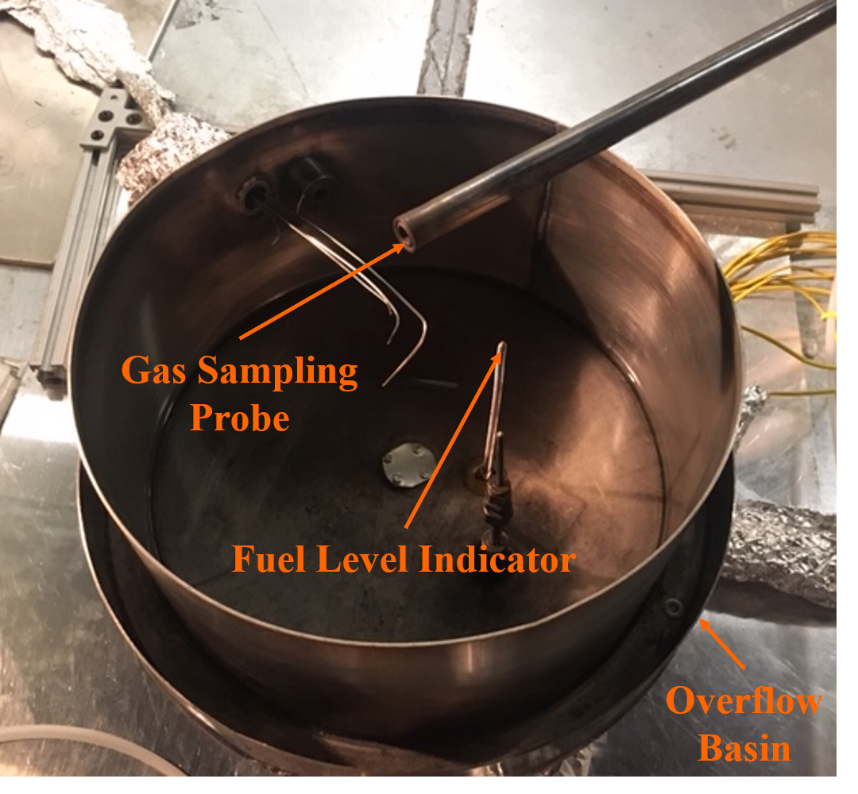
\includegraphics[width=10.0cm,keepaspectratio]{Pool_Burner.png}
	\caption[Pool Burner Design]{A 30~\si{cm} Pool Burner with fuel level indicator, overflow section, and quenching probe}
	\label{fig:Pool Burner}
\end{figure}

The time-averaged mass burning flux, $m''$, was determined from the rate at which fuel was delivered to the pool. Fuel to the burner was gravity fed from a reservoir positioned on a mass load cell located outside the enclosure and monitored by a data acquisition system. Figure~\ref{fig:Fuel_Level} shows the procedure for monitoring the fuel level via fuel flow operator. Using a live video feed, the operator was able to observe a close up of a slightly discernable dimple (Approximately 2~\si{mm}) made from the fuel level indicator on the fuel surface. The fuel level was controlled at 10~\si{mm} below the burner rim by manually adjusted the fuel flow using a needle valve.

The expanded uncertainty of the mass burning rate was estimated from a combination of Type A and B evaluation of standard uncertainty. The Type A evaluation of standard uncertainty was determined from the variance in the time-averaged mass burning flux measured during each test. The Type B evaluation of stnadard uncertainty was defined as the bias errors in the load cell used to measure the mass flux. The uncertainty of the mass burning flux is discussed further detail in Appendix~\ref{ssec:Mass_Burning_Rate}.

The heat release rate of each fuel, $\dot{Q}$, was calculated from Eq.\ref{eq:Heat_release_rate} using the time-averaged mass burning flux measurements:

\begin{equation}\label{eq:Heat_release_rate}
\dot{Q}= m''\Delta H_{c}A
\end{equation}
where $\Delta H_{c}$ is the heat of the combustion of the burned fuel provided by DIPPR\textsuperscript{\textregistered} and $A$ is the cross-sectional area of the pool fire. The uncertainty of the heat release rate was calculated from the law of propagation of uncertainty which is detaled in Appendix~\ref{ssec:Heat_Release_Rate}.

The mean flame height was estimated from 3600 frames obtained from high quality video recordings of the methanol, ethanol, and acetone pool fire tests. Frames were proccessed using MATLAB’s Image Processing Toolbox. Imported RGB images were decomposed into binary (black and white) images using a pre-set threshold level. The flame height for a single frame was defined as the distance between the pool surface and flame tip established using MATLAB software. The measurement was reapeated for each of the 3600 frames then averaged to provide the mean flame height. 

The uncertainty of the mean flame height was estimated by combing the Type A and B evaluation of uncertainty defined as the variance of the averaged height measurements from each frame and the bias error of the distance measured in each frame. A detailed description of the uncertainty analysis for the mean flame height is described in Appendix~\ref{ssec:Mean_Flame_Heigh}.

\begin{figure}[h!]
	\centering
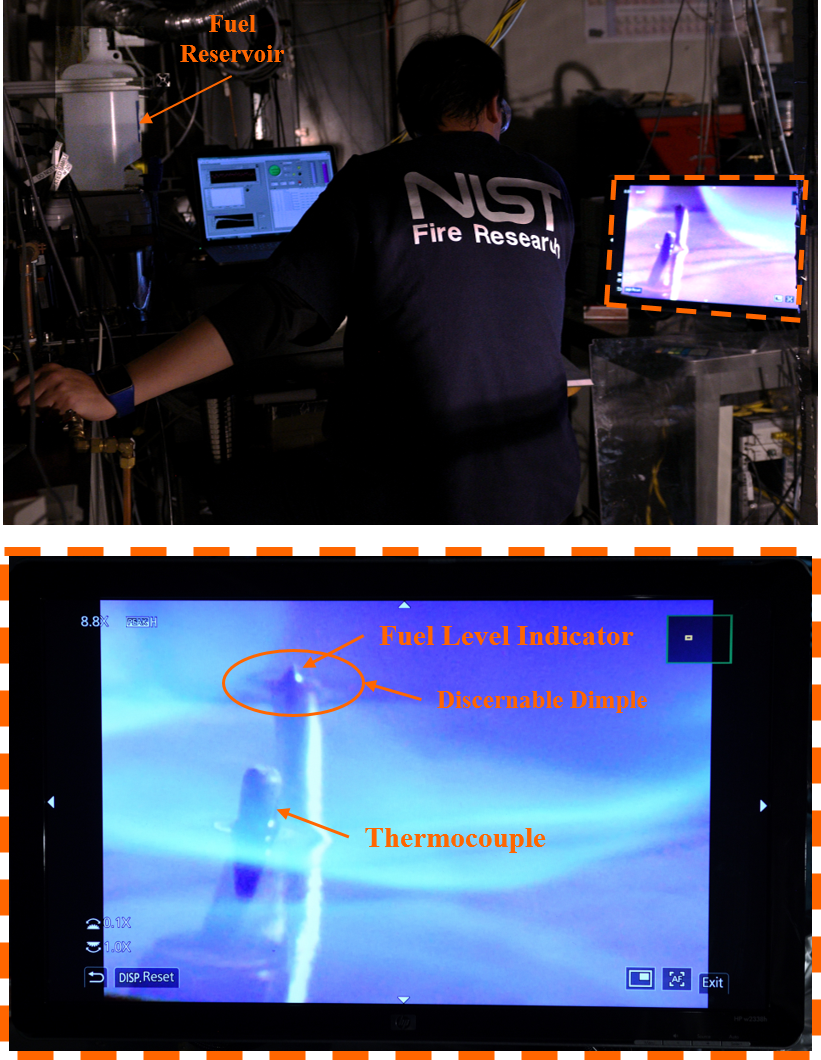
\includegraphics[width=14.0cm,keepaspectratio]{Monitoring_Fuel_Level_A.png}
	\caption[Monitoring Fuel Level]{Photo of fuel flow operators monitoring the fuel level via live video feed (top) and a close up image of the live video feed used to maintain a consistant fuel level relative to the fuel level indicator (bottom)}
	\label{fig:Fuel_Level}
\end{figure}
 
\subsection{Measuring the Volume Fraction of Gas Species via GC/MSD}
\label{ssec:Gas_Species_Setup}

Gas-species measurements were made using an Agilent 5977E Series GC/MSD fitted with a thermal conductivity detector (TCD). The GC/MSD was able to quantify a variety of stable reactants, intermediates, and combustion product species collected from the pool fire. The GC/MSD was equipped with a 2~\si{ml} sample loop maintained at a 200~°\si{C}. Chromatographic separation of species was achieved using a Select for Permanent Gases-Dual Column (CP7430) comprised of mole-sieve and Porapak Q columns working in parallel and using a helium carrier gas. The sample analysis time was 62~\si{min} wherein the carrier gas flow leading into the TCD and MSD was 3.00~\si{ml/min} and 1.00~\si{ml/min}, respectively. During the analysis, the GC oven temperature was maintained at 30~°\si{C} for 12~\si{min}, then ramped at 8~°\si{C}/\si{min} for 2~\si{min} until a temperature of 300~°\si{C} was obtained.

Figure~\ref{fig:Experimental_Setup} displays the flow diagram for gas sampling into the GC/MSD. After achieving steady-state burning conditions, approx. 10~\si{min} after ignition, flow prompted by a vacuum pump located downstream from the GC/MSD was initiated. Gas samples were collected using a quenching probe. The quenching probe was composed of two concentric, stainless-steel tubes with outer annular coolant flow and inner, extracted, gas-sample flow. The inner and outer tube diameters were 7.9~\si{mm} and 16~\si{mm}, respectively. Water at 90~°\si{C} flowed through the sampling probe for the duration of the experiment. The remainder of the sampling line leading into the GC/MSD was heated with electrical, heating tape to 140~°\si{C} to prevent condensation of water and liquid fuels through the line.

\begin{sidewaysfigure}[!]
	\centering
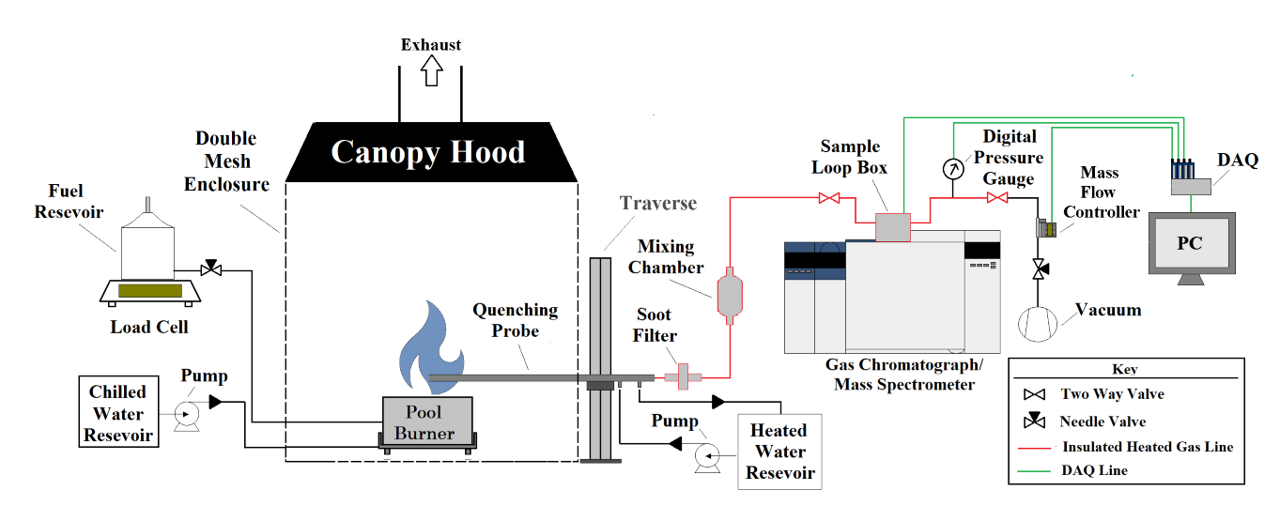
\includegraphics[width=\textwidth,keepaspectratio]{Experimental_Setup.png}
	\caption[A schematic of the gas sampling procedure]{A schematic of the extractive sampling setup used to transport gas samples from the pool fire to the GC/MSD}
	\label{fig:Experimental_Setup}
\end{sidewaysfigure}

Gas sampling was conducted for a minimum of 12~\si{min}, ensuring that the gas sample had completely swept through the GC/MSD sample loop. The gas sampling period varied from 12~\si{min} to 25~\si{min} depending on the sampling location within the fire. The sampling flow was controlled using a mass flow controller (Alicat Scientific MC-Series) located in front of the vacuum pump within the sampling line. During the gas sampling procedure, the volumetric flow was approximately 200~\si{ml/min} and recorded using DAQ at 2~\si{Hz} for the entire duration of the gas sampling procedure. The mass flow controlled also provided temperature readings of its internal gas flow.

After the gas sampling period, two quarter-turn valves located on opposite ends of the GC/MSD sample loop within the sampling line are closed. Once the sampled gas reached equilibrium, pressure measurements, obtained from a digital pressure gauge (OMEGA DPG409-030DWU), and temperature measurements, acquired by a K Type Thermocouple located at the GC/MSD Sample Loop injection port, were collected at 2~\si{Hz} for 50~\si{s}. After collecting pressure and temperature measurements, the sampled gas was injected into the GC/MSD.

The volume fraction, $\bar{X_{i}}$, was calculated from the ratio between the number of moles of a given gas species, $n_{i}$, and the total number of moles identified, $n_{tot}$. The moles of a given species were measured from the Thermal Conductivity Detector (TCD) within the GC/MSD. The total number of moles was determined from the summation of moles for each species identified by the TCD.

\begin{equation}\label{eq:volume_fraction}
  \bar{X_{i}}= \frac{n_{i}}{n_{tot}}
\end{equation}

The mass fraction, $\bar{Y_{i}}$, of each species $i$ was calculated from the measured volume fraction, $\bar{X_{i}}$, using the folowing expression:
\begin{equation}\label{eq:mass_fraction}
\bar{Y_{i}}=\frac{\bar{X_{i}}~{MW_{i}}}{{MW_{tot}}}
\end{equation}
where ${{MW_{i}}}$ is the molecular weight of a given species and ${{MW_{tot}}}$ is the average molecular weight of all detected gas species represented in the function below. 

 \begin{equation}\label{eq:Total_MW}
{MW_{tot}}=\sum{\bar{X_{i}}~{MW_{i}}}
\end{equation}

All measurements using the GC/MSD were repeated at least twice at each location along the centerline of the pool fire. Gas species concentration measurements made at the same location were averaged. The variance in the gas species volume fraction was a function of location and species. A detailed description of the uncertainty analysis for the gas species measurement and its calibration is discussed in Appendices~\ref{sec:UncertaintyGasSpecies} and \ref{sec:Uncertainty Analysis of Gas Species Calibrations}, respectively.

\subsection{Determining Soot Mass Fraction}
\label{ssec:Soot_Setup}

Soot was collected simultaneously with gas samples using the sampling procedure described in Section~\ref{ssec:Gas_Species_Setup}. Before a test, a dessicated 47~\si{mm} Polytetrafluoroethylene (PTFE) filter was weighed and subsequently placed into an in-line stainless steel particulate filter holder~\cite{GelmanSciences1235}. During a test, the filter holder was positioned within the gas sampling line behind the quenching probe and heated to 140~°\si{C} using heating tape to prevent condensation of water and liquid fuels on the filter. After testing, the PTFE filter was removed from the filter holder and dried in a desicator. After desicating for 48~\si{hrs}, the PTFE filter's final weight was measured. Approximately 2~\si{mg} of soot was collected during the gas sampling period which varied from 12~\si{min} to 25~\si{min} depending on the sampling location within the fire.

After some tests, soot deposits were observed on the inner walls of the quenching probe. As shown in Fig.~\ref{fig:Soot_Probe_Setup} desicated gun cleaning patches were used to clean the inside of the quenching probe. At least two patches were used to collect soot on the inside of the probe. Soot collection using patches concluded once a patch was observed to have no soot after being swept through the inner walls of the quenching probe. Patches were weighed immediately before and 48~\si{hrs} after cleaning the inside of the probe. The soot collected from the dry patches was accounted for when calculating the soot mass fraction. The portion of the soot collected on the inner walls of the quenching probe relative to the PTFE filter varied based on the sampling location. The mass of the PTFE filter and cleaning patches were measured three times before and after each test.

\begin{figure}[ht!]
	\centering
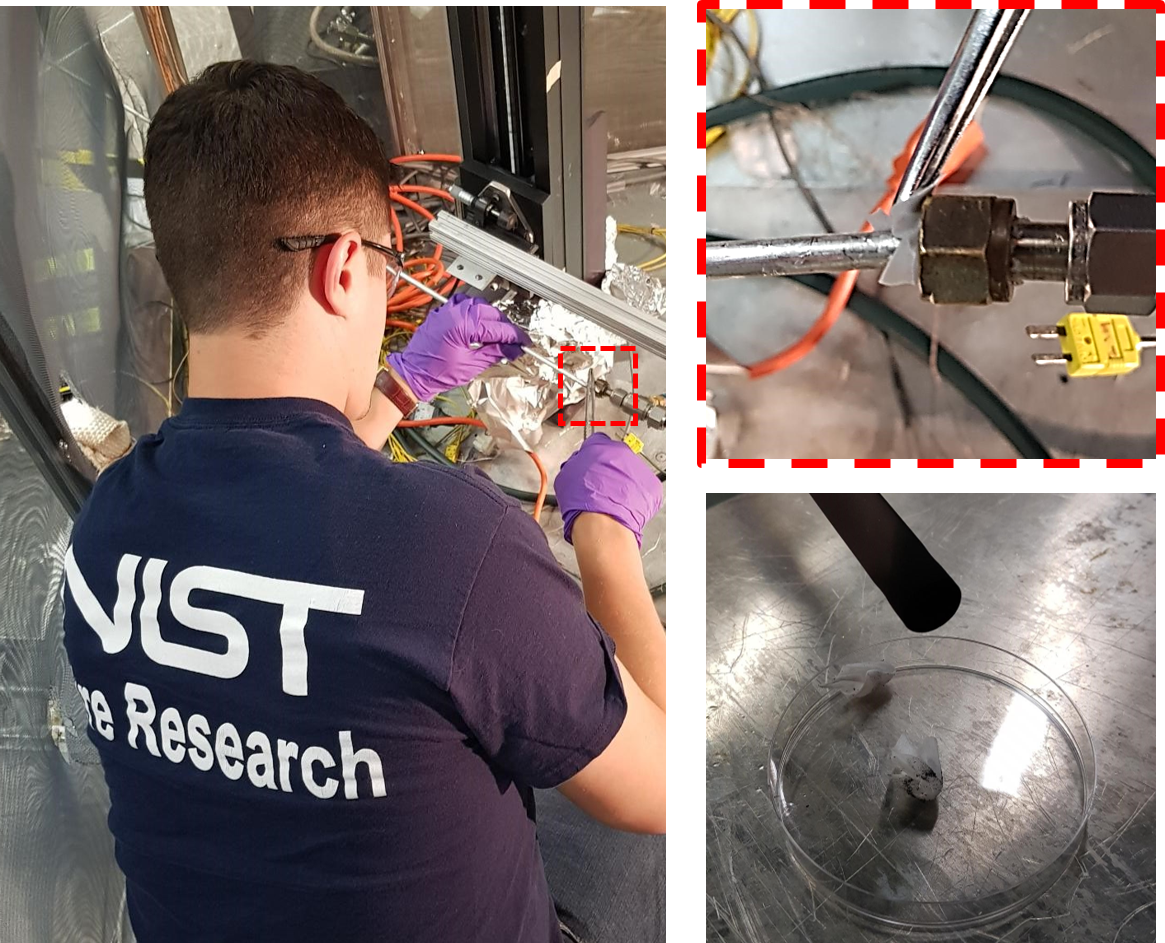
\includegraphics[width=15.0cm,keepaspectratio]{Soot_Probe.png}
	\caption[Process for cleaning soot probe]{Process of collecting soot from the internal walls of the quenching probe using gun cleaning patches}
	\label{fig:Soot_Probe_Setup}
\end{figure}

The soot mass fraction, $M_{s}$, was computed from the mass of the soot collected from the PTFE filter and gun cleaning patches, $m_{s}$, the ratio of the mass flow controller's temperature reading, $T_{\infty}$, to the temperature at the probe entrance,$T_{p}$, the total mass of gas sampled, $M_{t}$, based on the mass flow controller readings:

\begin{equation}\label{eq:soot_mass_frac}
  M_{s}= \frac{m_{s}}{M_{t}}\frac{T_{\infty}}{T_{p}}
\end{equation}
The total mass of gas sampled was estimated from product of the average volumetric flow rate measured by the mass flow controller, $\dot{V}$, the density of the sample gas injected into the GC/MSD, $\rho_{g}$, and the gas sampling time, $t$. 
\begin{equation}\label{eq:total_mass}
M_{t}= \dot{V}\cdot \rho_{g}\cdot t
\end{equation} 
In Eq.\ref{eq:total_mass}, the density of the sample gas was determined from the total mass detected in the TCD chromatogram, $m_{tot}$, for the injected sample volume, $V_{s}$. 
\begin{equation}\label{eq:gas_density}
\rho_{g}= \frac{m_{tot}}{V_{s}}
\end{equation} 

The uncertainty of the soot mass fraction was estimated from a combined uncertainty of the Type A evaluation of standard uncertainty in the variation of temperature and mass measurements and the Type B standard uncertainty in the bias errors of the instrumentation. A detailed description of the soot mass fraction uncertainty is provided in Appendix~\ref{sec:Uncertainty_Soot_Frac}.

\section{Mixture Fraction}
\label{sec:Mixture_Fraction}
The mixture fraction, $Z$, was based on carbon containing species and was defined as follows:
\begin{equation}\label{eq:Mixture_Fraction}
Z=Y_{F}+\frac{{MW_{F}}}{x}\sum{\frac{Y_{i}}{{MW_{i}}}}
\end{equation} 
where $Y_{F}$, ${MW_{F}}$, and $x$ are the mass fraction, molecular weight, and number of carbon molecules of the parent fuel, respectively. Considering the idealized reaction of a hydrocarbon fuel, the state reactions was derived as:
\begin{align*}
C_{x}H_{y}&O_{z}+\eta(x+\frac{y}{4}-\frac{z}{2})~(O_{2}+3.76~N_{2}+0.0445~Ar)\\
&\rightarrow max(0,1-\eta)~C_{x}H_{y}O_{z}+max(0,1-\eta)~(x+\frac{y}{4}~\frac{z}{2})~O_{2}+ min(1,\eta)~x~CO_{2}\\ 
&~~~~+min(1,\eta)~\frac{y}{2}~H_{2}O+\eta(x+\frac{y}{4}-\frac{z}{2})~(3.76~N_{2}+0.0445~Ar) \numberthis \label{eq:Ideal_rxn}
\end{align*}
where $max(\alpha,\beta)$ and $min(\alpha,\beta)$ are operators that return the larger and smaller value, respectively, of the two parameters $\alpha$ and $\beta$. The parameter $\eta$ represents the portion of air relative to the amount of fuel used as a reactant in Eq.~\ref{eq:Ideal_rxn}. In other words, $\eta$ can be defined as the reciprical of the local fuel equivalence ratio, $\phi$,
\begin{equation}\label{eq:Eta}
\phi=\frac{(F/A)}{(F/A)_{st}}=\frac{1}{\eta}
\end{equation} 
where $F/A$ is the fuel-air ratio and the subscript $st$ denotes the stoichiometric condition. The idealized mixture fractions of the products relative to the mixture fraction can then be calcuated through a combintation of Eq.~\ref{eq:Mixture_Fraction} and \ref{eq:Ideal_rxn}. 

The uncertainty of the mixture fraction was determined from propagating the error in the mass fraction measurements. A detailed description of the mixture fraction uncertainty is provided in Appendix~\ref{sec:Uncertainty_Mix_Frac}. 

\section{Results}
\label{sec:Results}
Brief observations of each pool fire burning different fuels are described in the first portion of this section. The key results of this work are the local gas species and soot measurements made at incremental heights along the centerline of medium-scale pool fires using various fuels such as methanol, ethanol, and acetone. A more in-depth analysis of the relationships between different measured gas is also provided in this section.

\subsection{Flame Observations}
\label{ssec:Flame_Observations}

Figure~\ref{fig:Flame_Structure} displays a series of snapshots depicting the flame pulsation of the methanol, ethanol, and acetone pool fires in the 30.0~\si{cm} stainless-steel water-cooled burned. A repeated cycle was observed in each of the pool fires; uniformly curved flame sheets present at the burner rim would roll towards the fire centerline to form a long and narrow plume.
\begin{figure}[!]
	\centering
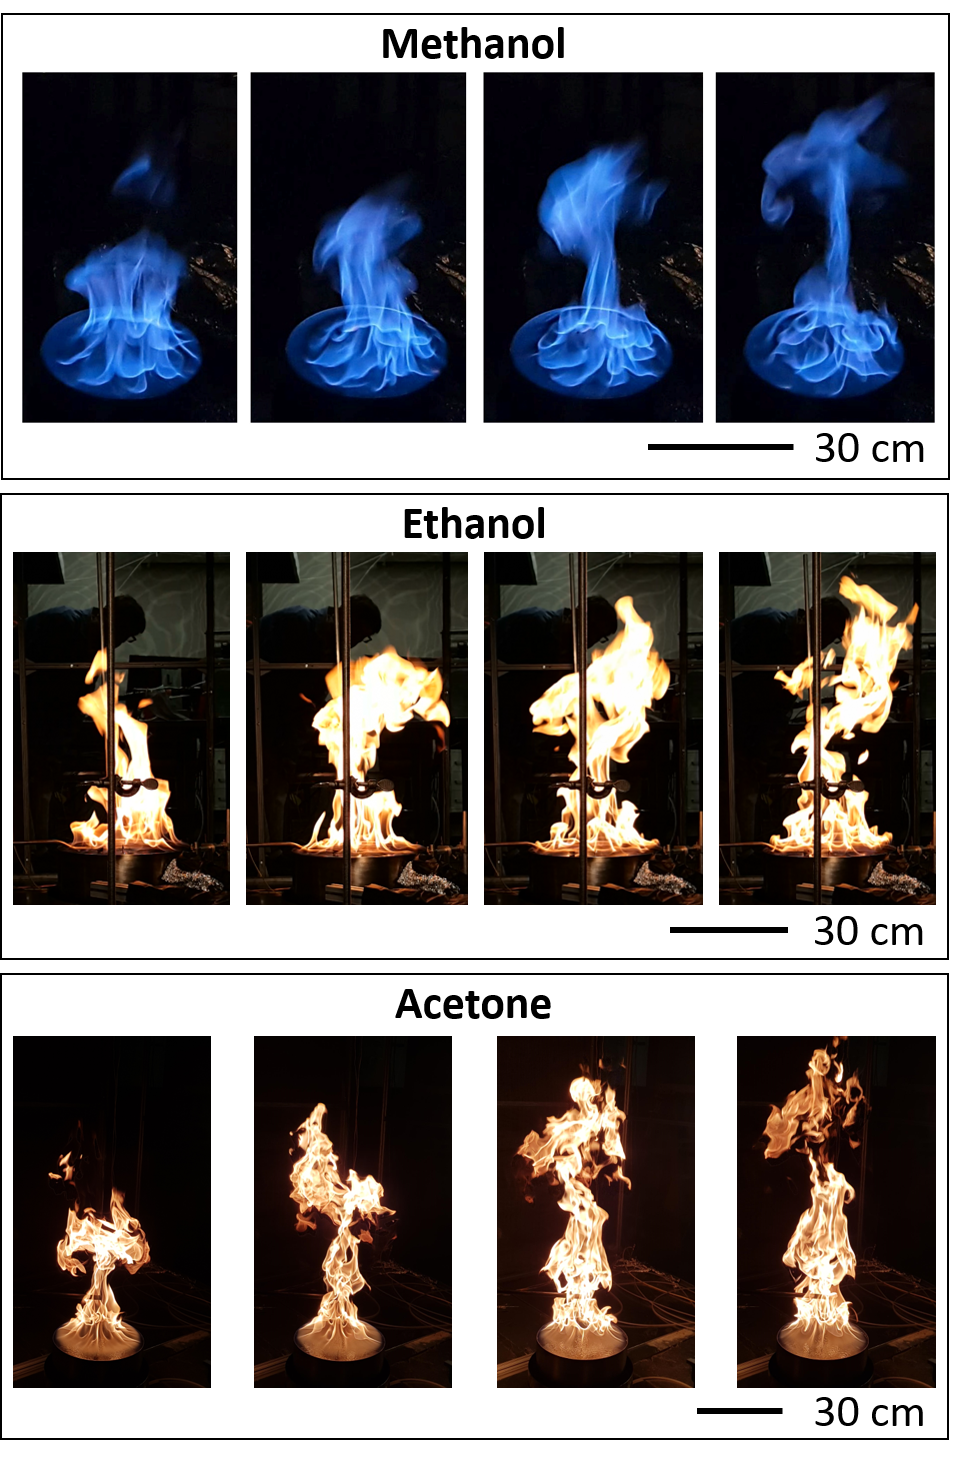
\includegraphics[width=12.0cm,keepaspectratio]{Flame_Structure.png}
	\caption[Pool Fire Structures]{Flame structures of methanol (top), ethanol (middle), and acetone (bottom) pool fires during their pulsing cycles}
	\label{fig:Flame_Structure}
\end{figure}

The shape and visible color of the fires differed between fuel types. The methanol fire appeared to be completely blue, whereas the ethanol and acetone fires primarily consisted of vibrant yellow and orange colors. The methanol pool fire was observed to exhibit a weak turbulent structure compared to the fully developed fires of the other two fuels. The observed dynamic shapes were consistent with previous experiments~\cite{Hamins2016,Hamins1994,Hamins1991,Hamins1996,Lock2008}. Table~\ref{tab:Pool_Fire_Parameters_Table} provides a list of measurements made of each pool fire. The observed provide in the Table below are consistent with previous works \cite{Kim2019}. 

\begin{table}[!]
\caption{List of measurements obtained in a well-ventilated round, steady, 30.0~\si{cm} diameter pool fire burning in a quiescent environment. The uncertainty of measurements of fire parameters are discussed in detail in Appendix~\ref{sec:Uncertainty_Pool_Fire_Parameters}.}
\label{tab:Pool_Fire_Parameters_Table}
\centering
	\footnotesize
	\begin{tabular}{lccc}
\hline
%\\[0.0005cm]
\textbf{Parameter (units)} &\textbf{Methanol}& \textbf{Ethanol}& \textbf{Acetone}\\
\hline
\\[0.01cm]
Mass Burning Flux~(\si{g/{m^2 s}})		&	12.4~$\pm$~1.1		&	13.9~$\pm$~0.8	&	17.6~$\pm$~2.7\\
\\[0.01cm]
Heat Release Rate~(\si{kW})			&	17.4~$\pm$~1.4		&	26.3~$\pm$~1.5	&	35.5~$\pm$~5.4\\
\\[0.01cm]
Mean Flame Height~(\si{cm})			&	40.5~$\pm$~14.8		&	61.1~$\pm$~28.2	&	87.3~$\pm$~32.8\\
%\\[0.01cm]
\hline
\end{tabular}
\end{table}

% Description of flame height calculation

% Description of mass burning flux

% Description of heat release rate

\subsection{Gas Species Concentrations}
\label{ssec:Gas_Species_Concentrations}

Figure~\ref{fig:Fuel_Comparison} displays the averaged volume fraction, $\bar{X_{i}}$, of significant species measurements made at various heights along the methanol, ethanol, and acetone fire centerlines. Significanat species detected in the TCD chromatogram include reactants, fuels and oxygen ($\chem{O_2}$), combustion products such as water ($\chem{H_2O}$) and carbon dioxide ($\chem{CO_2}$), combustion intermediates such as carbon monoxide ($\chem{CO}$), hydrogen ($\chem{H_2}$), methane ($\chem{CH_4}$), and inert gases such as Nitrogen ($\chem{N_2}$) and Argon ($\chem{Ar}$). 

%% Edit this paragraph
As expected, the fuel volume fractions were highest, and the oxygen volume fraction was the lowest close to the fuel surface. The product species were found to have a maximum volume fraction at approximately 4 cm above the fuel surface. The intermediate gas species were found to have peaked at approximately 2 cm above the fuel surface. Inert gases were shown to increase with the distance from the fuel surface. It was also found that the gas sampled from the centerline nearly mimicked the composition of air at approximately 60 cm above the fuel surface. 

\begin{figure}[!]
	\centering
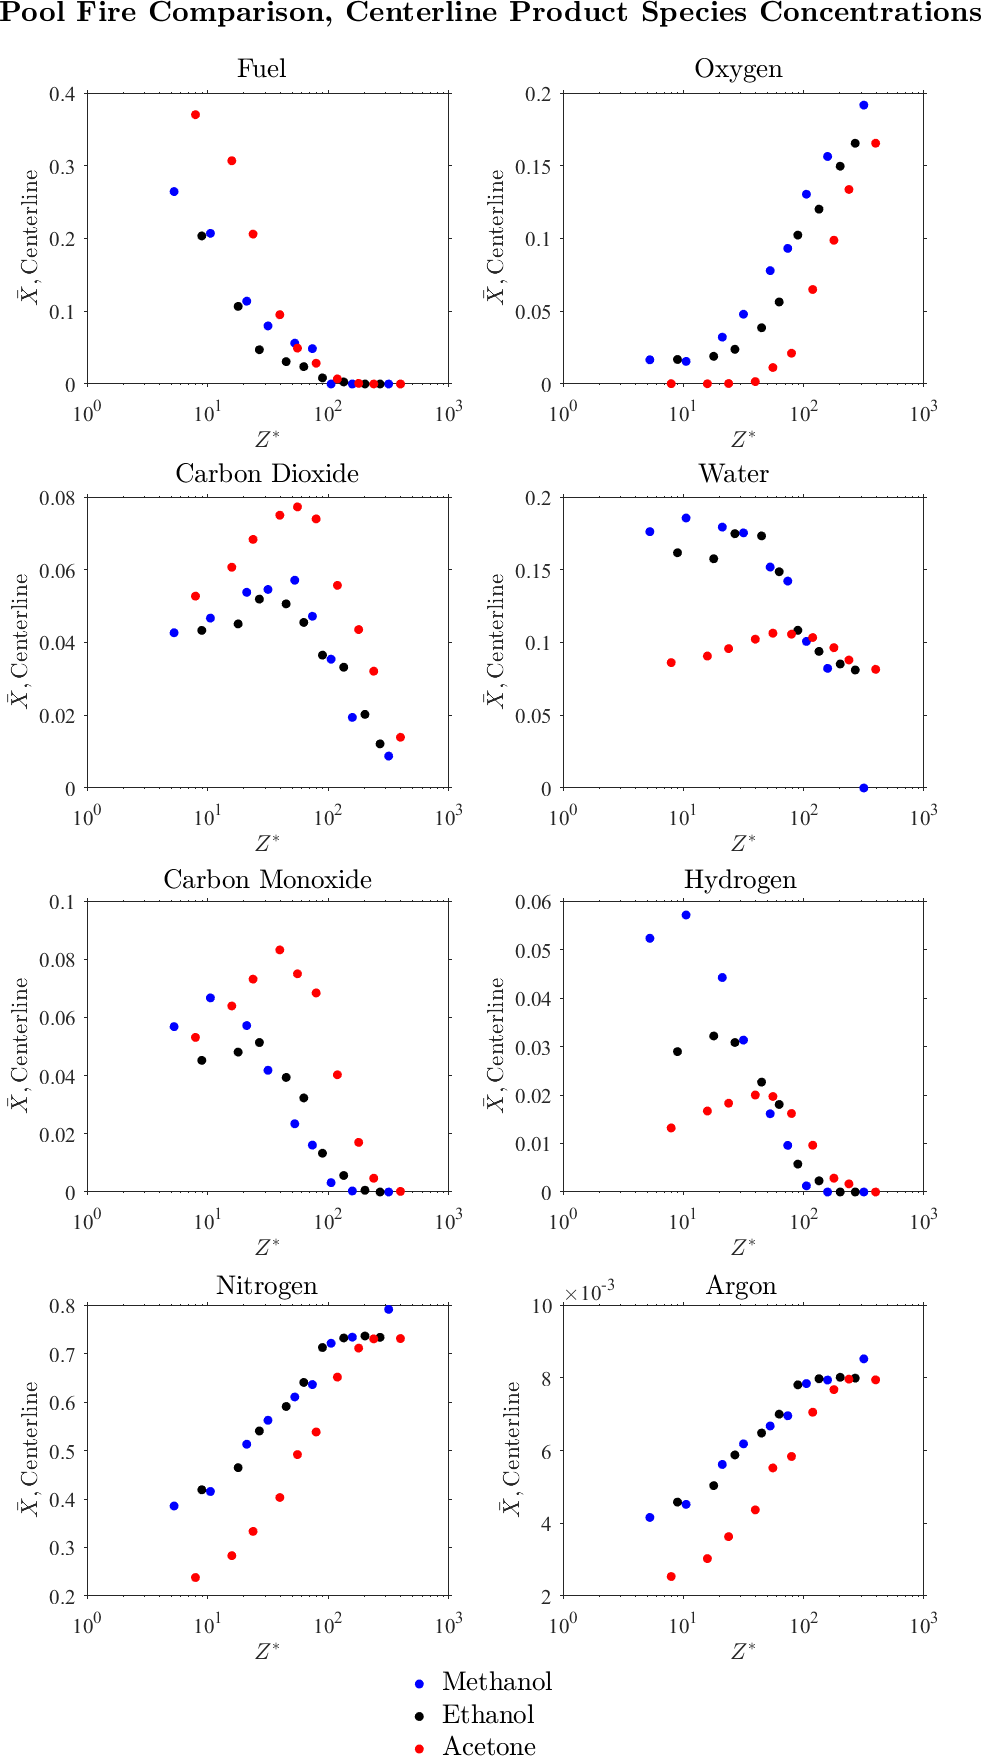
\includegraphics[width=12.0cm,keepaspectratio]{OVERALL_Fuel_Comparison.png}
	\caption[Major Species Comparison]{Flame structures of methanol (top), ethanol (middle), and acetone (bottom) pool fires during their pulsing cycles}
	\label{fig:Fuel_Comparison}
\end{figure}

\subsection{Soot Mass Fraction}
\label{ssec:Soot_Mass_Fraction}
%% Combine Soot Plots together; there is more soot for acetone than ethanol by an

\subsection{Mixture Fraction Results}
\label{ssec:Mixture_Fraction_Results}

\begin{figure}[!]
	\centering
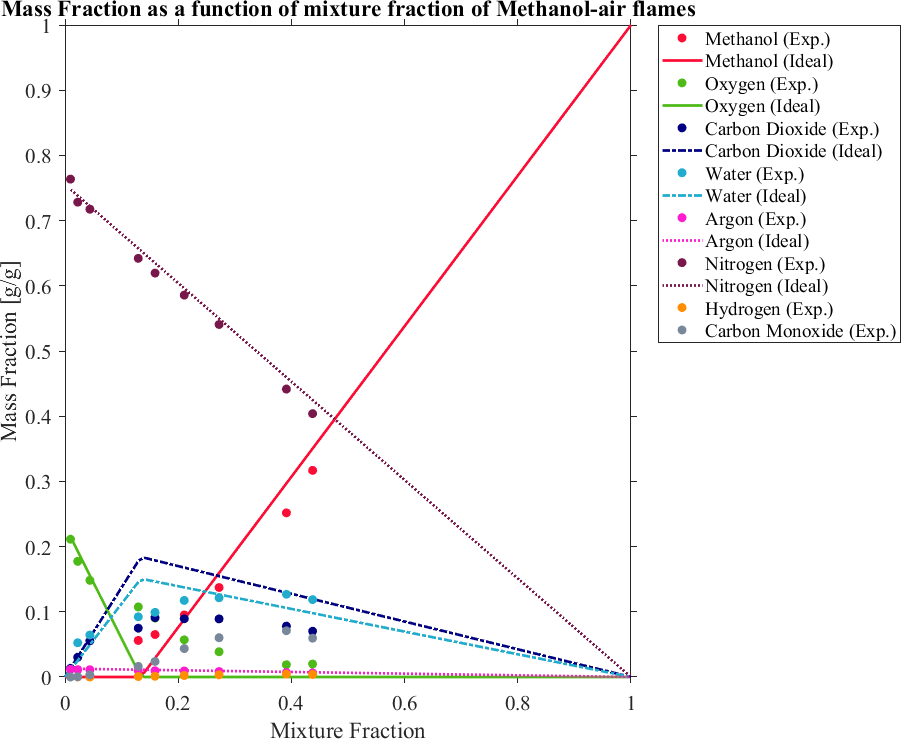
\includegraphics[width=12.0cm,keepaspectratio]{Methanol_Mass_Frac_Mix_Frac.png}
	\caption[Averaged quasi-steady mass fraction of major species as a function of mixture fraction for a methanol pool fire]{Mass fractions of major species detected from a methanol pool fire centerline as a function of mixture fracton}
	\label{fig:Methanol_Mix_Frac}
\end{figure}

\begin{figure}[!]
	\centering
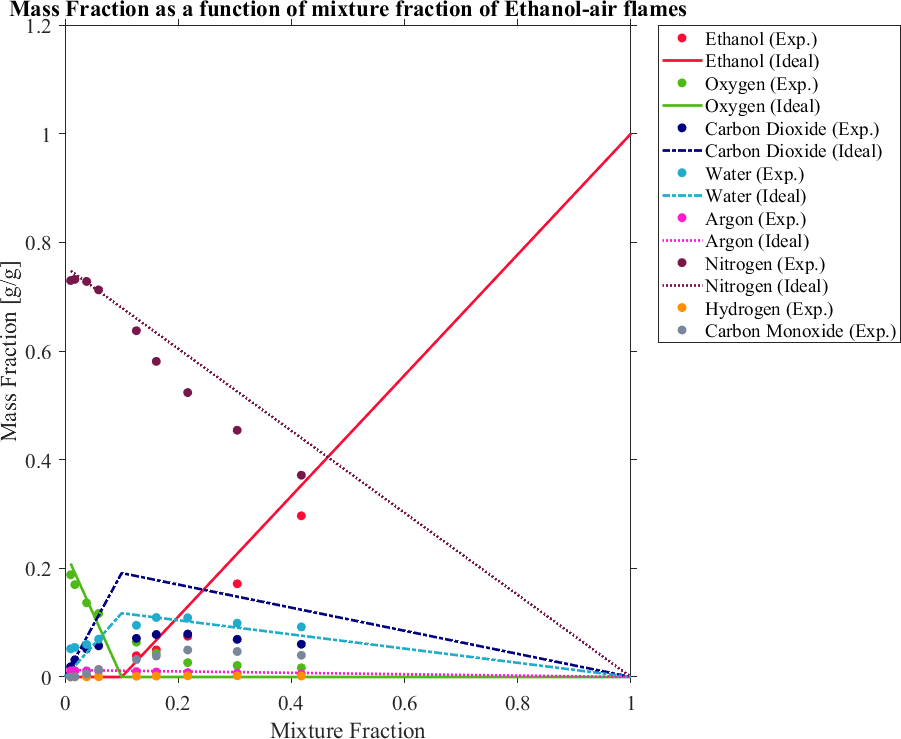
\includegraphics[width=12.0cm,keepaspectratio]{Ethanol_Mass_Frac_Mix_Frac.png}
	\caption[Averaged quasi-steady mass fraction of major species as a function of mixture fraction for an ethanol pool fire]{Mass fractions of major species detected from a ethanol pool fire centerline as a function of mixture fracton}
	\label{fig:Ethanol_Mix_Frac}
\end{figure}

\begin{figure}[!]
	\centering
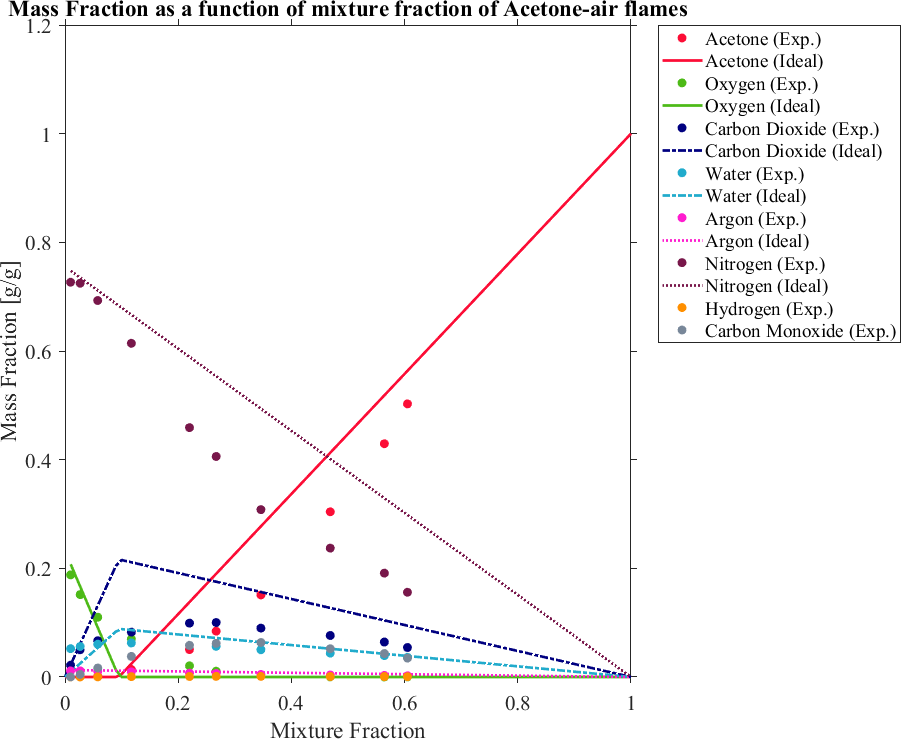
\includegraphics[width=12.0cm,keepaspectratio]{Acetone_Mass_Frac_Mix_Frac.png}
	\caption[Averaged quasi-steady mass fraction of major species as a function of mixture fraction for a acetone pool fire]{Mass fractions of major species detected from a acetone pool fire centerline as a function of mixture fracton}
	\label{fig:Acetone_Mix_Frac}
\end{figure}


\subsection{Carbon Balance}
\label{ssec:Carbon Balance}


\section{Conclusion}
\label{sec:Conclusion}

\section*{Acknowledgments}
\noindent The authors would like to acknowledge Kimberly Harris of the Gas Sensing Metrology Group at NIST, who assisted in the developing the species calibration method used in the study.

\pagebreak

\section*{References}
\addcontentsline{toc}{section}{References}
\bibliographystyle{techpubs}
\bibliography{References}


\pagebreak


\appendix
\numberwithin{equation}{section}
\makeatletter
% "activate" the preparatory code, but for section-level headers only
\newcommand{\section@cntformat}{Appendix:\ }
\makeatother

\section{Uncertainty Analysis of Gas Species Concentrations} \label{sec:UncertaintyGasSpecies}
\addcontentsline{toc}{section}{Appendix A: Uncertainty Analysis of Gas Species Concentrations}

As shown in Eq.~\ref{eq:volume_fraction}, volume fraction, $\bar{X_{i}}$ was calculated from the ratio between the number of moles of a given species, $n_{i}$, and the total number of moles identified, $n_{tot}$. The uncertainty of the measured volume fraction was estimated using the law of propagation of uncertainty after determining the volume fraction of each species:

\begin{equation}
\label{eq:Volume_Frac_Uncertainty}
u_\mathrm{\bar{X_{i}}} = \sqrt{{\left( \frac{\partial \bar{X_{i}}}{\partial n_{i}}\,u_{\scriptscriptstyle n_{i}} \right)}^2+{\left(\frac{\partial \bar{X_{i}}}{\partial n_{tot}}\,u_{\scriptscriptstyle n_{tot}}\right)}^2}
\end{equation}
A coverage factor of 2 was applied to the combined uncertainty to produce a 95~\% confidence interval.

\subsection{Number of Moles of a Given Species}
\label{ssec:Number_of_Moles_of_a_Given_Species}

The number of moles of a given species was determined from a calibration function of the integrated peak area of the respective species obtained from the TCD chromatogram. The Type A evaluation of standard uncertainty of the number of moles of a given species was taken as the standard deviation of the measurements obtained from the repeated tests. The Type B evaluation of standard uncertainty was determined from the error in the calibration functions for each species measured by the TCD further detailed in Appedix~\ref{sec:Uncertainty Analysis of Gas Species Calibrations}. The combined uncertainty was found via quadrature:

\begin{equation}
\label{eq:gasspeciesuncertaintycertainty}
u_{\scriptscriptstyle n_{i}} = \sqrt{ u_{\rm \scriptscriptstyle n_{i,cal}}^2 + s_{\scriptscriptstyle n_{i}}^2}
\end{equation}

\subsection{Total Number of Moles Identified}
\label{ssec:Total Number of Moles Identified}
The total number of moles detected was determined from the summation of the number of moles for each species identified by the TCD. Therefore, the uncertainty in the total number of moles identified was the combined uncertainty of all the identified species via quadrature:

\begin{equation}
\label{eq:totalnumberofmolesdetected}
u_{\scriptscriptstyle n_{tot}}=\sqrt{{\sum_{n=1}^{N} s_{\scriptscriptstyle n_{i}}^2}}
\end{equation}
where $N$ is the number of a species identified species in the TCD chromatogram. 

\pagebreak

\section{Uncertainty Analysis of Gas Species Calibrations}\label{sec:Uncertainty Analysis of Gas Species Calibrations}
\addcontentsline{toc}{section}{Appendix B: Uncertainty Analysis of Gas Species Calibrations}

A calibration function is a relationship between an integrated peak area on the TCD chromatogram, $Area_{i}$, and the number of moles of a given species injected into the GC/MSD, $n_{i}$. A calibration function was determined by injecting a known amount of moles of a given species into the GC/MSD, $n_{i,cal}$, and identifying the peak area corresponding to the individual species. For this work, the calibration functions are approximately linear consisting of a slope, $a$, and intercept, $b$.

\begin{equation}
\label{eq:Calibration Curve}
n_{i,cal} = a(Area_{i})+b
\end{equation}

Calibration functions were weighted to account for the error of each gas standard used in the calibration procedure. The uncertainty of a calibration function was determined using the law of propagation of uncertainty:

\begin{equation}
\label{eq:Given_Moles_Uncertainty}
 u_{\rm \scriptscriptstyle n_{i}} = \sqrt{{\left( \frac{\partial n_{i}}{\partial a}\,u_{\scriptscriptstyle a} \right)}^2+{\left(\frac{\partial {n_{i}}}{\partial b}\,u_{\scriptscriptstyle b}\right)}^2}
\end{equation}
The uncertainties of the slope and intercept in a weighting linear regression are as follows:
\begin{equation}
\label{eq:Slope_Uncertainty}
u_{\rm \scriptscriptstyle a} =\sqrt{\frac{\sum~\frac{1}{u_{n_{i,cal}}}}{(\sum~\frac{Area_{i}^2}{{u_{n_{i,cal}}^2}})(\sum~\frac{1}{{u_{n_{i,cal}}^2}})-(\sum~\frac{Area_{i}}{{u_{n_{i,cal}}^2}})^2}}
\end{equation}
\begin{equation}
\label{eq:Intercept_Uncertainty}
u_{\rm \scriptscriptstyle b} =\sqrt{\frac{\sum~\frac{Area_{i}^2}{u_{n_{i,cal}}}}{(\sum~\frac{Area_{i}^2}{{u_{n_{i,cal}}^2}})(\sum~\frac{1}{{u_{n_{i,cal}}^2}})-(\sum~\frac{Area_{i}}{{u_{n_{i,cal}}^2}})^2}}
\end{equation}
where $u_{n_{i,cal}}$ is the uncertainty of the known number of moles of the respective species.

During calibration, the number of moles of a given species $n_{i,cal}$ was calculated from the product of the total moles injected into the GC/MSD, $n_{tot,inj}$ and the known concentration of the particular species in the calibration standard, $C_{i}$.

\begin{equation}
\label{eq:Cal_Moles}
n_{i,cal} = C_{i}(n_{tot,inj})
\end{equation}
A collection of gas calibration standards for a variety of species were pre-selected to provide a broad range of concentrations. All calibration standards were mixtures of the target gas species with a Nitrogen balance, with the exception of one standard balanced in Air. A list of gas standards used in this work, with their respective concentrations and Type B evaluation of standard uncertainty, is provided in Appendix~\ref{sssec:Table of Gas Standards with Error}.

The uncertainty of the number of moles of a given species injected into the GC/MSD for calibration was estimated using the law of propagation of uncertainty:

\begin{equation}
\label{eq:Given_Moles_Cal_Uncertainty}
 u_{\rm \scriptscriptstyle n_{i,cal}} = \sqrt{{\left( \frac{\partial n_{i,cal}}{\partial C_{i}}\,u_{\scriptscriptstyle C_{i}} \right)}^2+{\left(\frac{\partial n_{i,cal}}{\partial n_{tot,inj}}\,u_{\scriptscriptstyle n_{tot,inj}}\right)}^2}
\end{equation}

\subsection{Total Moles Injected into the GC/MSD for Calibation}
\label{ssec:Total Moles Injected into the GC/MSD for Calibation}

The total moles injected into the GC/MSD for calibration was determined from the pressure, $P$, temperature, $T$, and volume, $V$, of the gas sample injected into the GC/MSD using the experimental setup described in Section~\ref{ssec:Gas_Species_Setup}. The injected sample was assumed to be an ideal gas: 
\begin{equation}
\label{eq:molesinjected}
n_{tot, inj} = \frac{PV}{RT}
\end{equation}
where $R$ is the universal gas constant (287~J/(mol $\cdot$K).

Pressure and temperature measurements were made using an Omega Digital Pressure Gauge (DPG409-030DWU) and K Type Thermocouple located at the GC/MSD Sample Loop injection valve, respectively, sampling at 2~\si{Hz} for 50~\si{s}. The volume of the GC/MSD sample loop, $V_{sl}$, was assumed to be 2~\si{ml}. The Type A evaluation of uncertainty of the total moles injected into the GC/MSD for calibration was determined from the standard error of the pressure, $s_{P}$, and temperature, $s_{T}$ readings from the sampling period. The Type B evaluation of uncertainty for the total moles injected into the GC/MSD for calibration is determined from the bias error sources in the instrumentation, $u_{inst}$, used to measure pressure (0.008\% accuracy of the reading), temperature (1.5~$^\circ$C), and volume (0.02 ml) of gas sample injected. The combined uncertainty of the pressure, temperature, and volume was found via quadrature:

\begin{equation}
\label{eq:pressure_uncertainty}
u_{\scriptscriptstyle P} = \sqrt{ u_{\rm \scriptscriptstyle inst}^2 + s_{\scriptscriptstyle P}^2}
\end{equation}
\begin{equation}
\label{eq:temp_uncertainty}
u_{\scriptscriptstyle T} = \sqrt{ u_{\rm \scriptscriptstyle inst}^2 + s_{\scriptscriptstyle T}^2}
\end{equation}
\begin{equation}
\label{eq:volume_uncertainty}
u_{\scriptscriptstyle V_{sl}} =\sqrt{ u_{\rm \scriptscriptstyle inst}^2}
\end{equation}
The standard uncertainty of the total moles injected into the GC/MSD for calibration was estimated using the law of propagation of uncertainty:
\begin{equation}
\label{eq:moles_injected_uncertainty}
u_{\scriptscriptstyle n_{tot,inj}} = \sqrt{{\left( \frac{\partial n_{tot,inj}}{\partial P}\,u_{\scriptscriptstyle P} \right) }^2+{\left(\frac{\partial n_{tot,inj}}{\partial T}\,u_{\scriptscriptstyle T}\right)}^2+{\left(\frac{\partial n_{tot,inj}}{\partial V_{sl}}\,u_{\scriptscriptstyle V_{sl}}\right)}^2}
\end{equation}

\pagebreak
\subsection{Table of Gas Standards with Error}
\label{sssec:Table of Gas Standards with Error}
A table of the gas standards with their respective concentrations and Type B evaluation of standard uncertainty, used for calibrating the GC/MSD is provided below. Lot numbers for all standards are provided for traceability.

\begin{table}[h!]

\caption{Gas Standards used to Calibrate GC/MSD}
\label{tab:Gas_Standards_Table}
\centering
	\footnotesize
	\begin{tabular}{lcll}
			\hline
%\\[0.0005cm]
\textbf{Components} &\textbf{Uncertainty(\%)}& \textbf{Distributor}	& \textbf{Lot No.}		\\
\hline
\\[0.001cm]
200 ppm Acetone		&	2.00	&	Gasco Affiliates, LLC. 		&	DNJ-ACE-200N-1		\\
0.26\% Acetylene		&	2.00	&	Gasco Affiliates, LLC.		&	FBJ-M24-0.25\%-1		\\
1.04\% Acetylene		&	2.00	&	Gasco Affiliates, LLC.		&	FBJ-M24-1		\\
1.02\% Argon		&	2.00	&	Gasco Affiliates, LLC.		&	DBJ-2-1N-1		\\
88.5\% Argon		&	2.00	&	Gasco Affiliates, LLC.		&	DBJ-2-90N-1		\\
100 ppm Benzene		&	2.00	&	Gasco Affiliates, LLC.		&	FBJ-21-100-3		\\
15.6\% Carbon Dioxide	&	0.04	&	NIST Gas Sensing Metrology Group		&	9-C-44		\\
24.5\% Carbon Dioxide	&	2.00	&	Gasco Affiliates, LLC. 		&	KBI-35-25-1		\\
1.00\% Carbon Dioxide	&	2.00	&	Matheson Tri-Gas		&	9306620888		\\
2.51\% Carbon Dioxide	&	2.00	&	Roberts Oxygen			&	1002080917		\\
7.00\% Carbon Dioxide	&	2.00	&	Roberts Oxygen			&	1009010318		\\
0.30\% Carbon Monoxide	&	2.00	&	Roberts Oxygen			&	1009010318			\\
9.00\% Carbon Dioxide	&	2.00	&	Praxair Doistribution Inc. 	&	304113044702		\\
0.02\% Carbon Monoxide	&	2.00	&	Matheson Tri-Gas		&	9306620888		\\
0.11\% Carbon Monoxide	&	2.00	&	Roberts Oxygen			&	1002080917		\\
4.00\% Carbon Monoxide	&	2.00	&	Praxair Doistribution Inc. 	&	304113044702		\\
7.81\% Carbon Monoxide	&	0.02	&	NIST Gas Sensing Metrology Group 		&	??????		\\
0.51\% Ethane		&	2.00	&	Gasco Affiliates, LLC.		&	FBJ-62N-0.5-1		\\
1.00\% Ethane		&	2.00	&	Gasco Affiliates, LLC.		&	FBJ-152N-1-1\%-1		\\
2.55\% Ethane		&	2.00	&	Gasco Affiliates, LLC.		&	FBJ-152N-2.5-1		\\
0.51\% Ethylene		&	2.00	&	Gasco Affiliates, LLC.		&	FBJ-62N-0.5\%-1		\\
1.02\% Ethylene		&	2.00	&	Gasco Affiliates, LLC.		&	FBJ-62N-1\%-1		\\
2.55\% Ethylene		&	2.00	&	Gasco Affiliates, LLC.		&	FBJ-62N-2.5\%-1		\\
0.26\% Hydrogen		&	2.00	&	Gasco Affiliates, LLC.		&	FBJ-84-0.25-1		\\
0.50\% Hydrogen		&	2.00	&	Gasco Affiliates, LLC.		&	KBI-84-0.5-1		\\
1.00\% Hydrogen		&	2.00	&	Gasco Affiliates, LLC.		&	KBI-84-1-3		\\
2.00\% Hydrogen		&	2.00	&	Gasco Affiliates, LLC.		&	FBJ-84-2-5		\\
4.03\% Hydrogen		&	2.00	&	Gasco Affiliates, LLC.		&	FBJ-84-4-2		\\
0.40\% Methane		&	2.00	&	Gasco Affiliates, LLC. 		&	DBJ-135N-0.4-1		\\
3.95\% Methane		&	2.00	&	Gasco Affiliates, LLC.		&	DBJ-135N-4-2		\\
40.8\% Methane		&	2.00	&	Gasco Affiliates, LLC.		&	DBJ-135N-40-1		\\
0.50\% Oxygen		&	2.00	&	Gasco Affiliates, LLC. 		&	DBJ-2-90N-1		\\
1.97\% Oxygen		&	0.01	&	NIST Gas Sensing Metrology Group		&	73-D-03		\\
5.02\% Oxygen		&	2.00	&	Gasco Affiliates, LLC.		&	DBJ-161-5-5		\\
9.92\% Oxygen		&	0.02	&	NIST Gas Sensing Metrology Group		&	72-D-60		\\
10.2\% Oxygen		&	2.00	&	Gasco Affiliates, LLC. 		&	KBI-161-10-6		\\
20.7\% Oxygen		&	0.04	&	NIST Gas Sensing Metrology Group		&	71-D-51		\\
0.42\% Propane		&	2.00	&	Gasco Affiliates, LLC.		&	DBJ-176N-0.4-1		\\
39.6\% Propane		&	2.00	&	Gasco Affiliates, LLC. 		&	DBJ-176N-40-1		\\
\\[0.005cm]
\hline
\end{tabular}
\end{table}

\pagebreak
\subsection{Concentration of Vapors from Bubblers}
\label{sssec:Concentration of Vapors from Bubblers}

Liquid material concentrations were calibrated from the ratio of the liquid-vapor pressure to the total pressure injected into the GC/MSD.

\begin{equation}
\label{eq:liquid_vapor_concentration}
C_{vap} =\frac {P_{vap}}{P}
\end{equation}

The vapor pressure of any given liquid can be calculated and modified using the bubbler setup shown in Fig.~\ref{fig:Bubbler}: 

\begin{figure}[h!]
	\centering
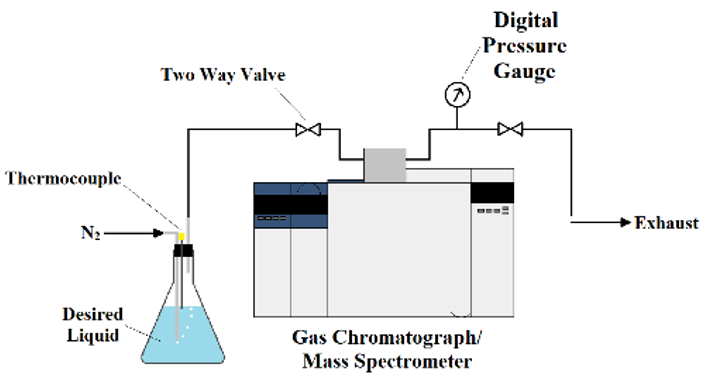
\includegraphics[width=\textwidth,keepaspectratio]{Bubbler_Setup.png}
	\caption[Flow diagram for bubble calibration system used for liquid materials]{Flow diagram for bubble calibration system used for liquid materials (acetone, ethanol, methanol, and water)}
	\label{fig:Bubbler}
\end{figure}
Nitrogen, acting as a carrier gas, was bubbled at the bottom of a liquid bath which after reaching the liquid surface transport vapor molecules through a heated gas line and into the GC/MSD sample loop. The concentration of the vapor injected into the GC/MSD was calculated from a liquid-vapor pressure correlation provided by DIPPR\textsuperscript{\textregistered}.

\begin{equation}
\label{eq:liquid_vapor_pressure_correlation}
P_{vap} =e^{A+\frac{B}{T}+C~\ln{T}+D~T^{E}}
\end{equation}
In this correlation, $P_{vap}$ is the vapor pressure calculated from the temperature of the liquid bath, $T$, with the coefficients ($A$, $B$, $C$, $D$, $E$) specific to the liquid material. Table~\ref{tab:Liquid Calibrate_Table} lists all coefficients for each calibrated liquid, including the uncertainty of their respective correlations, $u_{corr}$. 

\begin{table}[!]
\caption{Liquid Vapor Pressure Correlation Coefficients for Various Calibrated Liquids}
\label{tab:Liquid Calibrate_Table}
\centering
	\footnotesize
	\begin{tabular}{lcccccc}
			\hline
%\\[0.0005cm]
\textbf{Liquid Material} &\textbf{A}& \textbf{B}& \textbf{C}&\textbf{D}&\textbf{E}&\textbf{Uncertainty(\%)}\\
\hline
\\[0.001cm]
Acetone	&	69.006	&	-5599.6	&	-7.0985	&	6.2237E-6	& 	2.00	&  3.00\\
Ethanol	&	73.304	&	-7122.3	&	-7.1424	&	2.8853E-6	& 	2.00	&  1.00\\
Methanol	&	82.718	&	-6904.5	&	-8.8622	&	7.4664E-6	& 	2.00	&  3.00\\
Water		&	73.649	&	-7258.2	&	-7.3037	&	4.1653E-6	& 	2.00	&  0.20\\
\\[0.01cm]
\hline
\end{tabular}
\end{table}

The concentration range of each calibrated liquid typically spanned between 2~\% and 50~\%. Liquid bath temperatures were controlled using a heating plate positioned underneath the insulated bubbler. The temperature of the bath, $T_{b}$, was measured using a K Type thermocouple placed at the liquid bath's surface. The liquid bath temperature measurements were sampled at 2~\si{Hz} for 50~\si{s} simultaneously with pressure and temperature measurements of the GC/MSD sample loop. Liquid-vapor calibrations were conducted once the bath a steady-state temperature (approximately 1 hour) and the Nitrogen/vapor gas mixture has swept through the GC/MSD sample loop. Upon injection into the GC/MSD, pressure and temperature measurements of the sample loop are made as previously describe in Appendix~\ref{ssec:Total Moles Injected into the GC/MSD for Calibation}.

The uncertainty of the concentration determined using Eq.~\ref{eq:liquid_vapor_concentration} was estimated using the law of propagation of uncertainty:
\begin{equation}
\label{eq:vapor_concentration_uncertainty}
u_{\scriptscriptstyle C_{vap}} = \sqrt{{\left( \frac{\partial C_{vap}}{\partial P}\,u_{\scriptscriptstyle P} \right) }^2+{\left(\frac{\partial C_{vap}}{\partial P_{vap}}\,u_{\scriptscriptstyle P_{vap}}\right)}^2}
\end{equation}

The uncertainty of the pressure measured upon injected was calculated from Eq.~\ref{eq:pressure_uncertainty}. The uncertainty of the vapor pressure was found by combining the propagated error of liquid bath temperauture and the uncertainty in the correlation via quadrature:

\begin{equation}
\label{eq:vapor_concentration_uncertainty}
u_{\scriptscriptstyle P_{vap}} = \sqrt{{\left(\frac{\partial P_{vap}}{\partial T_{B}}\,u_{\scriptscriptstyle T_{B}} \right)}^2+{u_{corr}}^2}
\end{equation} 

The Type A evaluation of uncertainty of the liquid bath temperautre readings is determined from the standard error of the temperature, $s_{T_{B}}$ readings from the sampling period. The Type B evaluation of uncertainty for the liquid bath temperature was the bias error source (1.5~$^\circ$C) in the thermocouple, $u_{inst}$. The combined uncertainty liquid bath temperature was determined via quadrature:

\begin{equation}
\label{eq:temp_bath_uncertainty}
u_{\scriptscriptstyle T_{B}} = \sqrt{u_{\rm \scriptscriptstyle inst.}^2 + s_{\scriptscriptstyle T_{B}}^2}
\end{equation}


\pagebreak

\section{Uncertainty Analysis of the Soot Mass Fraction} \label{sec:Uncertainty_Soot_Frac}
\addcontentsline{toc}{section}{Appendix C: Uncertainty Analysis of the Soot Mass Fraction}
The local soot mass fraction measurements, $M_{s}$ made at various heights above the fuel surface in pool fires of different fuels were calculated through a combination of Eq.~\ref{eq:soot_mass_frac}, \ref{eq:total_mass}, and \ref{eq:gas_density}:
\begin{equation}\label{eq:overall_soot_mass_frac}
 M_{s}= \frac{m_{s}~V_{sl}}{\dot{V}~t~m_{tot}}\frac{T_{\infty}}{T_{p}}
\end{equation}
where $m_{s}$ is the mass of soot collected on the PTFE filter and gun cleaning patches, $\dot{V}$ is the volumetric flow rate measured by the mass flow controller, $V_{sl}$ is the volume of the sample loop, $\sum~n_{i}\cdot{MW_{i}}$ is the total mass of the gas sample detected in the TCD chromatogram calculated from the summation of the product of the number of moles of a given species and their respective molar mass, $T_{\infty}/T_{p}$ is the ratio of the internal gas flow temperature readings of the mass flow controller to the temperature of the probe, and $t$ is the total sampling time. The uncertainty of the measured soot mass fraction was estimated using the law of propagation of uncertainty after determing the soot mass fraction:

\begin{equation}
\label{eq:soot_mass_frac_uncertainty}
u_{\scriptscriptstyle M_{s}} = \sqrt{{\left(\frac{\partial M_{s}}{\partial m_{s}}\,u_{\scriptscriptstyle m_{s}} \right)}^2+{\left(\frac{\partial M_{s}}{\partial \dot{V} }\,u_{\scriptscriptstyle \dot{V}} \right)}^2+{\left(\frac{\partial M_{s}}{\partial V_{sl}}\,u_{\scriptscriptstyle V_{sl}} \right)}^2+{\left(\frac{\partial M_{s}}{\partial m_{tot}}\,u_{\scriptscriptstyle m_{tot}} \right)}^2+{\left(\frac{\partial M_{s}}{\partial T_{\infty}}\,u_{\scriptscriptstyle T_{\infty}} \right)}^2+{\left(\frac{\partial M_{s}}{\partial T_{p}}\,u_{\scriptscriptstyle T_{p}} \right)}^2}
\end{equation}
A coverage factor of 2 was applied to the combined uncertainty to produce a 95~\% confidence interval.

\subsection{Mass of Soot}
\label{ssec:Mass_of_Soot}

The mass of soot was measured from the difference in mass of a dried PTFE filter and dried gun cleaning patches immediately before and 48~\si{hrs} after each test. The Type A evaluation of standard uncertainty of the mass of soot, $m_{s}$ was taken as the standard deviation, $s_{m_{s}}$, of the measurements sampled three times before and after each test. The Type B evaluation of Uncertainty was determined from the instraumentation error sources of the scale and was found to be $u_{inst}=$~1\% of the reading. The combined uncertainty was found via quadrature:

\begin{equation}
\label{eq:soot_mass_uncertainty}
u_{\scriptscriptstyle m_{s}} = \sqrt{u_{\rm \scriptscriptstyle inst}^2 + s_{\scriptscriptstyle m_{s}}^2}
\end{equation}

\subsection{Mass Flow Controller Volumetric Flow Rate}
\label{ssec:Mass_Flow_Controller_Volumetric_Flow_Rate}

A mass flow controller was used to measure the volumetric flow rate, $\dot{V}$, within the gas sampling line. The Type A evaluation of standard uncertainty was taken as the standard deviation of the flow measurements sampled at 2~\si{Hz} during the gas sampling period which varied from12~\si{min} to 25~\si{min} depending on the sampling location within the fire. The Type B evaluation of standard uncertainty was determined from the calibration error, $u_{cal}$, and the precision error sources at calibration conditions, $u_{p}$, defined as $2~\si{ml}$ and 0.8~\% of the reading + 0.2~\% of the full scale ($2~\si{Lpm}$), respectively. The combined uncertainty is calculated via quadrature:

\begin{equation}
\label{eq:volumetric_flow_uncertainty}
u_{\scriptscriptstyle \dot{V}} = \sqrt{u_{\rm \scriptscriptstyle p}^2 + u_{\rm \scriptscriptstyle cal}^2 + s_{\scriptscriptstyle \dot{V}}^2}
\end{equation}

\subsection{GC/MSD Sample Loop Volume}
\label{ssec:Sample_Loop_Volume}

All gas sampling experiments and calibrations were conducted using a 2~\si{ml} sampling loop. The Type B evaluation of standard uncertainty of the GC/MSD sample loop volume was assumed to be 1~\%. \footnote{The uncertainty of the sample loop was assumed to be 1~\% after contacting the manufacturer.}

\subsection{Total Mass Injected into the GC/MSD}
\label{ssec:Total_Mass_Injected_into_GC/MSD}
The total mass detected in the TCD chromatogram, $m_{tot}$, was calculated from the summation of products of the moles of given species and their respective molar mass,${MW_{i}}$: 

\begin{equation}
\label{eq:total_mass_detected_uncertainty}
m_{tot}=\sum_{n=1}^{N}  n_{i}\cdot{MW_{i}}
\end{equation}

The uncertainty in the total mass detected was defined as the combined uncertainty of all identified species multiplied by their corresponding molar mass via quadrature:

\begin{equation}
\label{eq:total_mass_detected_uncertainty}
u_{\scriptscriptstyle m_{tot}}=\sqrt{{\sum_{n=1}^{N} (s_{\scriptscriptstyle n_{i}}\cdot{MW_{i}})^2}}
\end{equation}
where $N$ is the number of a species identified species in the TCD chromatogram. 

\subsection{Mass Flow Controller Internal Gas Flow Temperature Reading}
\label{ssec:MFC_Temp}

The mass flow controller provides an internal gas flow temperature reading that was recorded manually during the gas sampling process. The uncertainty of the temperature reading was determined from the Type B evaluation of standard uncertainty of the mass flow controller temperature measurement defined as 0.75~\% of the reading.

\subsection{Temperature Reading at the Entrance of the Probe}
\label{ssec:Probe_Temp}

\pagebreak

\section{Uncertainty Analysis of the Mixture Fraction}\label{sec:Uncertainty_Mix_Frac}
\addcontentsline{toc}{section}{Appendix D: Uncertainty of the Mixture Fraction}
The mixture fraction, $Z$ was determined from Eq.\ref{eq:Mixture_Fraction} based on carbon containing species. The uncertainty of the determined mixture fraction was estimated using the law of propagation of uncertainty based on calculated mass fractions, $Y_{i}$. 

\begin{equation}
\label{eq:mixture_frac_uncertainty}
u_{\scriptscriptstyle Z}=\sqrt{{\sum_{i=1}^{N}{\left(\frac{\partial Z}{\partial Y_{i}}\,u_{\scriptscriptstyle Y_{i}} \right)}^2}}
\end{equation}

\pagebreak

\section{Uncertainty Analysis of Pool Fire Parameters}\label{sec:Uncertainty_Pool_Fire_Parameters}
\addcontentsline{toc}{section}{Appendix E: Uncertainty of Pool Fire Parameters}

\subsection{Mass Burning Rate}
\label{ssec:Mass_Burning_Rate}

\subsection{Heat Release Rate}
\label{ssec:Heat_Release_Rate}

\subsection{Mean Flame Height}
\label{ssec:Mean_Flame_Height}

\pagebreak

\end{document}
